% !Mode:: "TeX:UTF-8"
\documentclass{article}
\usepackage[UTF8,zihao=-4]{ctex}                     % 支持中文显示
\usepackage{graphicx}                       % 支持插图处理
% 支持版面尺寸设置
\usepackage{titlesec}                       % 控制标题的宏包
\usepackage{titletoc}                       % 控制目录的宏包
\usepackage{fancyhdr}                       % fancyhdr宏包 支持页眉和页脚的相关定义
\usepackage{color}                          % 支持彩色
\usepackage{amsmath}                        % AMSLaTeX宏包 用来排出更加漂亮的公式
\usepackage{amssymb}                        % 数学符号生成命令
\usepackage[below]{placeins}                %允许上一个section的浮动图形出现在下一个section的开始部分,还提供\FloatBarrier命令,使所有未处理的浮动图形立即被处理
\usepackage{flafter}                        % 使得所有浮动体不能被放置在其浮动环境之前,以免浮动体在引述它的文本之前出现.
\usepackage{multirow}                       % 使用Multirow宏包,使得表格可以合并多个row格
\usepackage{booktabs}                       % 表格,横的粗线;\specialrule{1pt}{0pt}{0pt}
\usepackage{longtable}                      % 支持跨页的表格。
\usepackage{tabularx}                       % 自动设置表格的列宽
\usepackage{subfigure}                      % 支持子图 %centerlast 设置最后一行是否居中
\usepackage[subfigure]{ccaption}            % 支持子图的中文标题
\usepackage[sort&compress,numbers]{natbib}  % 支持引用缩写的宏包
\usepackage{enumitem}                       % 使用enumitem宏包,改变列表项的格式
\usepackage{calc}                           % 长度可以用+ - * / 进行计算
\usepackage{txfonts}                        % 字体宏包
\usepackage{bm}                             % 处理数学公式中的黑斜体的宏包
\usepackage[amsmath,thmmarks,hyperref]{ntheorem}  % 定理类环境宏包,其中 amsmath 选项用来兼容 AMS LaTeX 的宏包
%如果您的pdf制作中文书签有乱码使用如下命令,就可以解决了
\usepackage{hyperref}
%%%%%%%%%%%%%%算法环境%%%%%%%%%%%%%%
\usepackage{listings}
\usepackage{xcolor}
\definecolor{dkgreen}{rgb}{0,0.6,0}
\definecolor{gray}{rgb}{0.5,0.5,0.5}
\definecolor{mauve}{rgb}{0.58,0,0.82}
\lstset{
	backgroundcolor=\color{gray!5},
	basicstyle={\linespread{1.1}\footnotesize\ttfamily},
	breakatwhitespace=true,
	breaklines=true,
	commentstyle=\color{dkgreen},
	frame=single,
	frameshape={RYRYNYYYY}{yny}{yny}{RYRYNYYYY},
	keywordstyle=\color{blue},
	language=Python,
	numbers=none,
	numberstyle=\tiny\color{gray},
	rulecolor=\color{gray!35},
	showstringspaces=false,
	stringstyle=\color{mauve},
	tabsize=4,
	aboveskip=3mm,
	belowskip=3mm,
	columns=flexible,
	framerule=1pt,
}
%%%%%%%%%%%%%%算法环境%%%%%%%%%%%%%%
%%%%%%%%%%%%去除目录红框%%%%%%%%%%%%
\hypersetup{
	colorlinks=true,
	linkcolor=black,
}
%%%%%%%%%%%%去除目录红框%%%%%%%%%%%%
%%%%%%%%%%%%%调整页边距%%%%%%%%%%%%%
\usepackage{geometry}
\geometry{a4paper,left=2cm,right=2cm,top=2cm,bottom=2cm}
%%%%%%%%%%%%%调整页边距%%%%%%%%%%%%%
\usepackage{appendix}










\begin{document}

\title{图像处理作业——图像分割}
\author{刘坤鑫\thanks{3017218061 软件工程一班}}
\date{\today}
\maketitle
\begin{abstract}
本文对高斯拉普拉斯(LoG)进行了数学推导;简要介绍了最小二乘法、多项式最小二乘法的原理,给出了一种基于矩阵运算的高效实现;剖析了Python第三方包scikit-learn、scikit-image、scipy源码,在此基础上实现了RANSAC、霍夫变换算法;对于上述算法,以人工制造的数据和一张真实桌子图像sobel算子提取的边缘图像做对比分析。
\end{abstract}

\section{LoG的推导}

二维高斯函数表达式如下:

\begin{equation}
G(x, y)=\mathrm{e}^{-\frac{x^{2}+y^{2}}{2 \sigma^{2}}}
\end{equation}

拉普拉斯算子表达式如下:

\begin{equation}
\nabla^{2} = \frac{\partial^2 }{\partial x^2} + \frac{\partial^2 }{\partial y^2}
\end{equation}

故高斯拉普拉斯(LoG)可推导如下:

\begin{equation}
\begin{aligned} \nabla^{2} G(x, y) &=\frac{\partial^{2} G(x, y)}{\partial x^{2}}+\frac{\partial^{2} G(x, y)}{\partial y^{2}} \\ &=\frac{\partial}{\partial x}\left[\frac{-x}{\sigma^{2}} \mathrm{e}^{-\frac{x^{2}+y^{2}}{2 \sigma^{2}}}\right]+\frac{\partial}{\partial y}\left[\frac{-y}{\sigma^{2}} \mathrm{e}^{-\frac{x^{2}+y^{2}}{2 \sigma^{2}}}\right] \\ &=\left[\frac{x^{2}}{\sigma^{4}}-\frac{1}{\sigma^{2}}\right] \mathrm{e}^{-\frac{x^{2}+y^{2}}{2 \sigma^{2}}}+\left[\frac{y^{2}}{\sigma^{4}}-\frac{1}{\sigma^{2}}\right] \mathrm{e}^{-\frac{x^{2}+y^{2}}{2 \sigma^{2}}} \\ &=\left[\frac{x^{2}+y^{2}-2 \sigma^{2}}{\sigma^{4}}\right] e^{-\frac{x^{2}+y^{2}}{2 \sigma^{2}}} \end{aligned}
\end{equation}

\section{线性回归模型}

\subsection{最小二乘法}

最小二乘法是回归分析中的一种标准方法,通过最小化每个方程的残差平方和来逼近超定方程组(方程多于未知数的方程组)的解。

考虑线性方程组:

\begin{equation}
	\left[\begin{array}{cccc}{1} & {x_{1,1}} & {\ldots} & {x_{1,m}} \\ {1} & {x_{2,1}} & {\ldots} & {x_{2,m}} \\ {\ldots} & {\ldots} & {\ldots} & {\ldots} \\ {1} & {x_{n,1}} & {\ldots} & {x_{n,m}}\end{array}\right]\left[\begin{array}{c}{w_{0}} \\ {w_{1}} \\ {\ldots} \\ {w_{m}}\end{array}\right]=\left[\begin{array}{c}{y_1} \\ {y_2} \\ {\ldots} \\ {y_{n}}\end{array}\right]
\end{equation}

记为:

\begin{equation}\label{euqa:1}
	X\cdot w^T=y
\end{equation}

其中$x_{i,j}$表示第$i$个样本的第$j$元属性。最小二乘法试图确定最佳的$w$和$y$,使得拟合出来的直线尽量符合样本数据。

考虑均方误差(MSE)作为性能的度量,我们试图优化:

\begin{equation}
\begin{aligned}
\hat{w}^{*}&=\underset{\hat{w}}{\arg \min }(y-\hat{y})^2 \\ 
&=\underset{\hat{w}}{\arg \min }(y-X\hat{w})^2 \\
&= \underset{\hat{w}}{\arg \min }(y-{X} \hat{{w}})^{\mathrm{T}}({y}-{X} \hat{{w}})
\end{aligned}
\end{equation}

令$E_{\hat{{w}}}=({y}-\mathbf{X} \hat{{w}})^{\mathrm{T}}({y}-\mathbf{X} \hat{{w}})$,对$\hat{w}$求导得到:

\begin{equation}
\frac{\partial E_{\hat{{w}}}}{\partial \hat{{w}}}=2 {X}^{{T}}({X} \hat{{w}}-{y})
\end{equation}

令上式为零可得$\hat{w}$最优解的闭式解:

\begin{equation}
\hat{{w}}^{*}=\left({X}^{{T}} {X}\right)^{-1} {X}^{{T}} {y}
\end{equation}

这里为了简单起见,我们假定$X^TX$为满秩矩阵(full-rank matrix)或正定矩阵(positive definite matrix),即$(X^TX)^{-1}$有解。

求出$\hat{w}$,$y$也可以由式\ref{euqa:1}得出。

Python代码:

\begin{lstlisting}[title={最小二乘法代码}]
class LinearLeastSquare(object):
    def fit(self, X, y):
        X = np.hstack((np.ones((X.shape[0], 1)), X))
        self.W = np.linalg.inv(X.T.dot(X)).dot(X.T).dot(y)
        return self

    def predict(self, X):
        X = np.hstack((np.ones((X.shape[0], 1)), X))
        y = X.dot(self.W)
        return y

    def score(self, X, y):
        y_pred = self.predict(X)
        MSE = np.mean((y-y_pred)**2)
        return MSE
\end{lstlisting}

\subsection{多项式最小二乘法}

普通最小二乘法不能处理非线性的情况,但只要稍加改进,即可处理非线性的情况。

令

\begin{equation}
	X^{(k)}=\left[\begin{array}{cccc} x_{1,1}^k & x_{1,2}^k & {\ldots} & x_{1,m}^k \\ x_{2,1}^k & x_{2,2}^k & {\ldots} & x_{2,m}^k \\ {\ldots} & {\ldots} & {\ldots} & {\ldots} \\ x_{n,1}^k & x_{n,2}^k & {\ldots} & x_{n,m}^k\end{array}\right]
\end{equation}

\begin{equation}
	w^{(k)}=\begin{bmatrix}
	w_{k*m+1}\\ 
	w_{k*m+2}\\ 
	\ldots\\ 
	w_{k*m+m}
	\end{bmatrix}
\end{equation}

考虑方程组:

\begin{equation}
	\sum_{k=0}^{D}\limits X^{(k)} w^{(k)}=y
\end{equation}

其中,$D$为多项式最高次幂。

可见上式仍未线性方程组,可用普通最小二乘法或者任意一个线性回归模型解决。

Python代码:

\begin{lstlisting}[title={多项式最小二乘法代码}]
class PolynomialLeastSquares(object):
    def __init__(self, degree=3, base_estimator=LinearLeastSquare):
        self.degree = degree
        self.base_estimator = base_estimator()

    def fit(self, X, y):
        new_X = np.zeros(shape=(X.shape[0], 0))
        for i in range(self.degree):
            new_X = np.hstack((new_X, X**(i+1)))
        self.base_estimator.fit(new_X, y)
        self.W = self.base_estimator.W
        return self

    def predict(self, X):
        new_X = np.zeros(shape=(X.shape[0], 0))
        for i in range(self.degree):
            new_X = np.hstack((new_X, X**(i+1)))
        y = self.base_estimator.predict(new_X)
        return y

    def score(self, X, y):
        y_pred = self.predict(X)
        MSE = np.mean((y-y_pred)**2)
        return MSE
\end{lstlisting}

\subsection{RANSAC}

代码参考sklearn源码\footnote{\url{https://github.com/scikit-learn/scikit-learn/blob/master/sklearn/linear\_model/\_ransac.py}}。

\begin{lstlisting}[title={RANSAC代码}]
class RANSAC(object):
    def __init__(self,
                 base_estimator=LinearLeastSquare,
                 min_samples=None,
                 residual_threshold=None,
                 max_trials=100):
        self.base_estimator = base_estimator()
        self.min_samples = min_samples
        self.residual_threshold = residual_threshold
        self.max_trials = max_trials

    def fit(self, X, y):
        if self.min_samples is None:
            # assume linear model by default
            self.min_samples = X.shape[1] + 1

        if self.residual_threshold is None:
            # MAD (median absolute deviation)
            self.residual_threshold = np.median(np.abs(y - np.median(y)))

        n_inliers_best = 1
        score_best = np.inf
        inlier_mask_best = None
        X_inlier_best = None
        y_inlier_best = None

        sample_idxs = np.arange(X.shape[0])

        for i in range(self.max_trials):
            # choose random sample set
            all_idxs = np.arange(X.shape[0])
            np.random.shuffle(all_idxs)
            subset_idxs = all_idxs[:self.min_samples]

            # fit model for current random sample set
            self.base_estimator.fit(X[subset_idxs], y[subset_idxs])
            y_pred = self.base_estimator.predict(X)

            # residuals of all data for current random sample model
            residuals_subset = np.sum(np.abs(y-y_pred), axis=1)

            # classify data into inliers and outliers
            inlier_mask_subset = residuals_subset < self.residual_threshold
            n_inliers_subset = np.sum(inlier_mask_subset)

            # less inliers -> skip current random sample
            if n_inliers_subset < n_inliers_best:
                continue

            # extract inlier data set
            inlier_idxs_subset = sample_idxs[inlier_mask_subset]
            X_inlier_subset = X[inlier_idxs_subset]
            y_inlier_subset = y[inlier_idxs_subset]

            # score of inlier data set
            score_subset = self.base_estimator.score(
                X_inlier_subset, y_inlier_subset)

            # same number of inliers but worse score -> skip current random
            if (n_inliers_subset == n_inliers_best and score_subset > score_best):
                continue

            # save current random sample as best sample
            n_inliers_best = n_inliers_subset
            score_best = score_subset
            inlier_mask_best = inlier_mask_subset
            X_inlier_best = X_inlier_subset
            y_inlier_best = y_inlier_subset

        # estimate final model using all inliers
        self.base_estimator.fit(X_inlier_best, y_inlier_best)
        self.inlier_mask_ = inlier_mask_best
        return self

    def predict(self, X):
        return self.base_estimator.predict(X)

    def score(self, X, y):
        return self.base_estimator.score(X, y)
\end{lstlisting}

\subsection{数据处理}

按照题目要求,对于某条直线,y轴数据服从高斯分布,即x轴也服从正态分布,然后人工添加离群点。代码如下:

\begin{lstlisting}[title={数据处理}]
def make_data(n_samples=1000, n_inputs=1, n_outputs=1, noise=0.1, n_outliers=50):
    X = np.random.normal(size=(n_samples, n_inputs))
    W = np.ones(shape=(n_inputs, n_outputs))
    y = X.dot(W) + noise*np.random.normal(size=(n_samples, n_outputs))
    X[:n_outliers] = 3 + np.random.normal(size=(n_outliers, n_inputs))
    y[:n_outliers] = 0.5 + noise*np.random.normal(size=(n_outliers, n_outputs))
    return X, y
\end{lstlisting}

\subsection{结果展示}

\begin{figure}[ht]
	\centering
	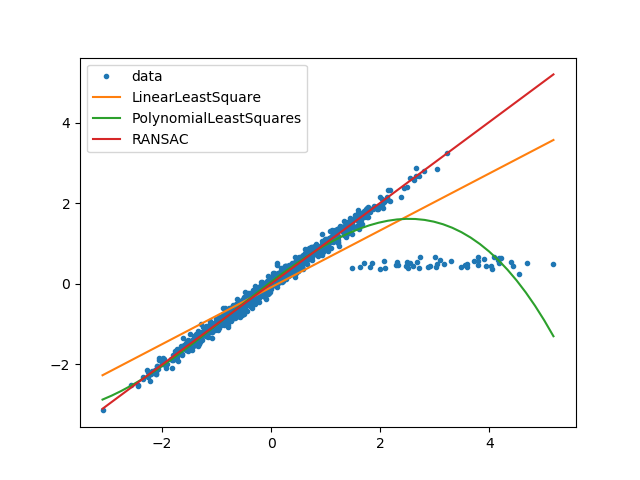
\includegraphics{../code/img/LinearRegression.png}
	\caption{三种线性回归模型拟合效果}
	\label{fig:Lr}
\end{figure}

如图\ref{fig:Lr}为三种线性回归模型拟合效果。其中,最小二乘法对于离群点敏感,多项式最小二乘法过拟合,RANSAC有效解决了离群点的问题,增强了鲁棒性。

\section{霍夫变换}

\subsection{原理}

参考博文``霍夫变换 - 疯狂奔跑 - 博客园''\footnote{\url{https://www.cnblogs.com/php-rearch/p/6760683.html}}。

\subsection{实现}

参考skimage源码\footnote{\url{https://github.com/scikit-image/scikit-image/blob/master/skimage/transform/\_hough\_transform.pyx}}

\begin{lstlisting}[title={hough transform}]
def hough_line(img):
    # Rho and Theta ranges
    thetas = np.deg2rad(np.arange(-90.0, 90.0))
    width, height = img.shape
    diag_len = int(np.ceil(np.sqrt(width * width + height * height)))   # Dmax
    rhos = np.linspace(-diag_len, diag_len, diag_len * 2.0)
    # Cache some resuable values
    cos_t = np.cos(thetas)
    sin_t = np.sin(thetas)
    num_thetas = len(thetas)
    # Hough accumulator array of theta vs rho
    accumulator = np.zeros((2 * diag_len, num_thetas), dtype=np.uint64)
    y_idxs, x_idxs = np.nonzero(img)  # (row, col) indexes to edges
    # Vote in the hough accumulator
    for i in range(len(x_idxs)):
        x = x_idxs[i]
        y = y_idxs[i]
        for t_idx in range(num_thetas):
            # Calculate rho. diag_len is added for a positive index
            rho = int(round(x * cos_t[t_idx] + y * sin_t[t_idx]) + diag_len)
            accumulator[rho, t_idx] += 1
    return accumulator, thetas, rhos
\end{lstlisting}

\begin{figure}[ht]
	\centering
	\subfigure[原始数据]{
		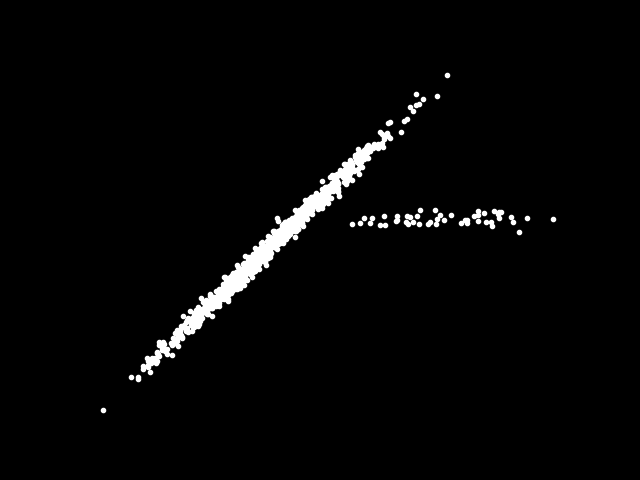
\includegraphics[height=6.5cm]{../code/img/data.png}
		%\caption{fig1}
	}
	\quad
	\subfigure[数据在霍夫空间]{
		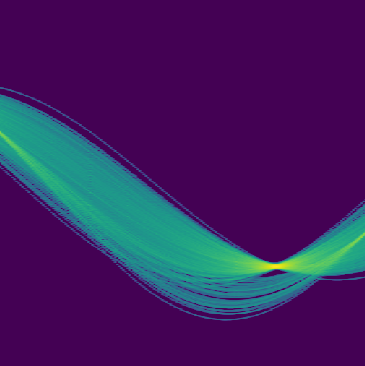
\includegraphics[height=6.5cm]{../code/img/hough_transform.png}
	}
	\caption{霍夫变换}
	\label{fig:data}
\end{figure}

如图\ref{fig:data}为前文人工制造的数据。左图为原始数据,右图为数据在霍夫空间中的形态。因为霍夫变换适合在一张图像上进行操作,所以把题一的数据转换为图像格式。

由图可知,笛卡尔坐标中的一条直线代表霍夫空间中的一个点,霍夫空间中越亮的点,说明重叠次数越多,即在笛卡尔坐标中直线相交越多,这样的直线越有可能是要检测的边缘。

\begin{figure}[ht]
	\centering
	\subfigure[threshold=50]{
		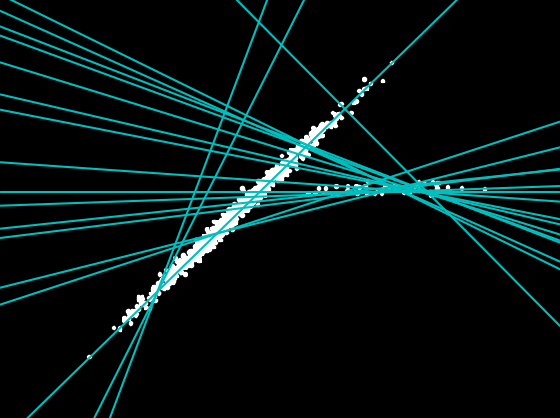
\includegraphics[width=7cm]{../code/img/hough_line50.png}
		%\caption{fig1}
	}
	\quad
	\subfigure[threshold=100]{
		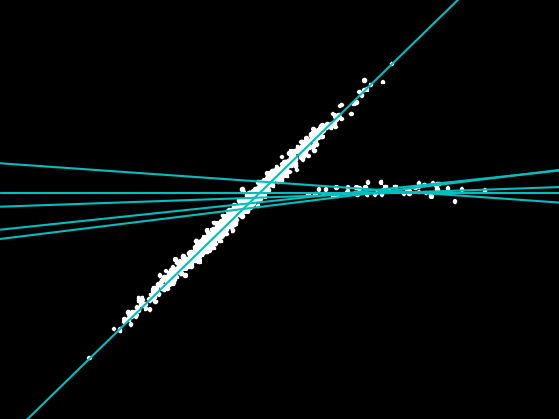
\includegraphics[width=7cm]{../code/img/hough_line100.png}
	}
	\\
	\subfigure[threshold=130]{
		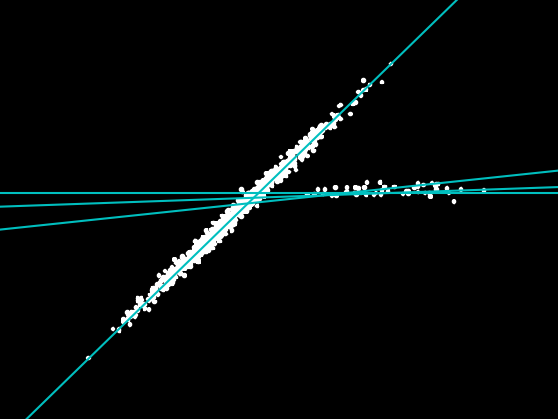
\includegraphics[width=7cm]{../code/img/hough_line130.png}
	}
	\quad
	\subfigure[threshold=150]{
		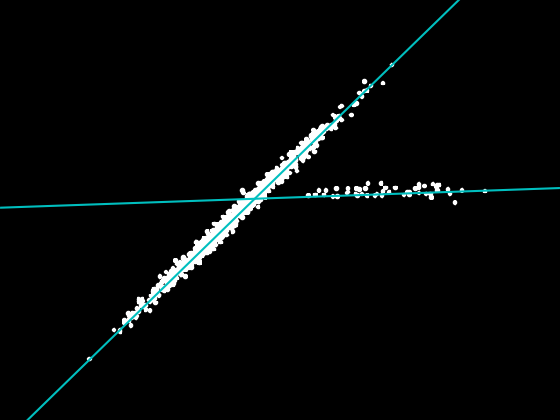
\includegraphics[width=7cm]{../code/img/hough_line150.png}
	}
	\caption{霍夫直线不同的阈值的结果图}
	\label{fig:hough-line}
\end{figure}

如图\ref{fig:hough-line}为霍夫直线不同的阈值的结果图。在霍夫变换中,对于每个点的每个$\theta$进行一次投票,最后可以得到计数的总和,计数越多,越有可能成为一条直线。阈值的作用在于筛选出计数大于阈值的直线。阈值越大,直线越少。

下面为求解霍夫变换空间和霍夫直线的代码:

\begin{lstlisting}[title={hough space and hough line}]
def show_transform(accumulator, path):
    image = np.log(1+accumulator)
    image = transform.resize(image, (512, 512))
    plt.imshow(image)
    plt.axis('off')
    plt.savefig(os.path.join('img', path))
    plt.close()


def show_line(image, accumulator, thetas, rhos, threshold, path):
    io.imshow(image)
    row, col = image.shape
    for _, angle, dist in zip(*transform.hough_line_peaks(accumulator, thetas, rhos, threshold=threshold)):
        y0 = (dist - 0 * np.cos(angle)) / np.sin(angle)
        y1 = (dist - col * np.cos(angle)) / np.sin(angle)
        plt.plot((0, col), (y0, y1), '-c')
    plt.axis((0, col, row, 0))
    path = os.path.join('img', path+str(threshold))
    plt.savefig(path)
    plt.close()
\end{lstlisting}

\subsection{更多结果展示}

\begin{figure}[ht]
	\centering
	\subfigure[桌子]{
		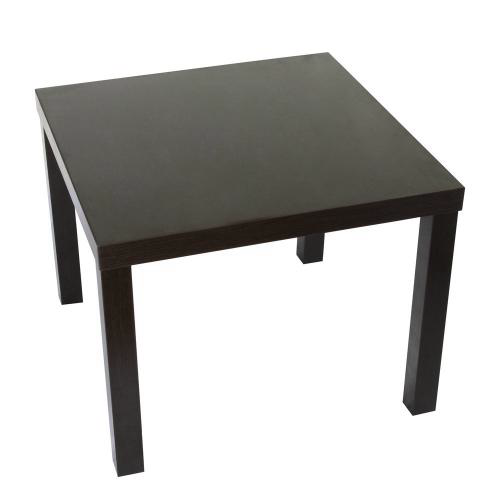
\includegraphics[height=6.5cm]{../code/img/desk.png}
		%\caption{fig1}
	}
	\quad
	\subfigure[桌子sobel算子边缘提取]{
		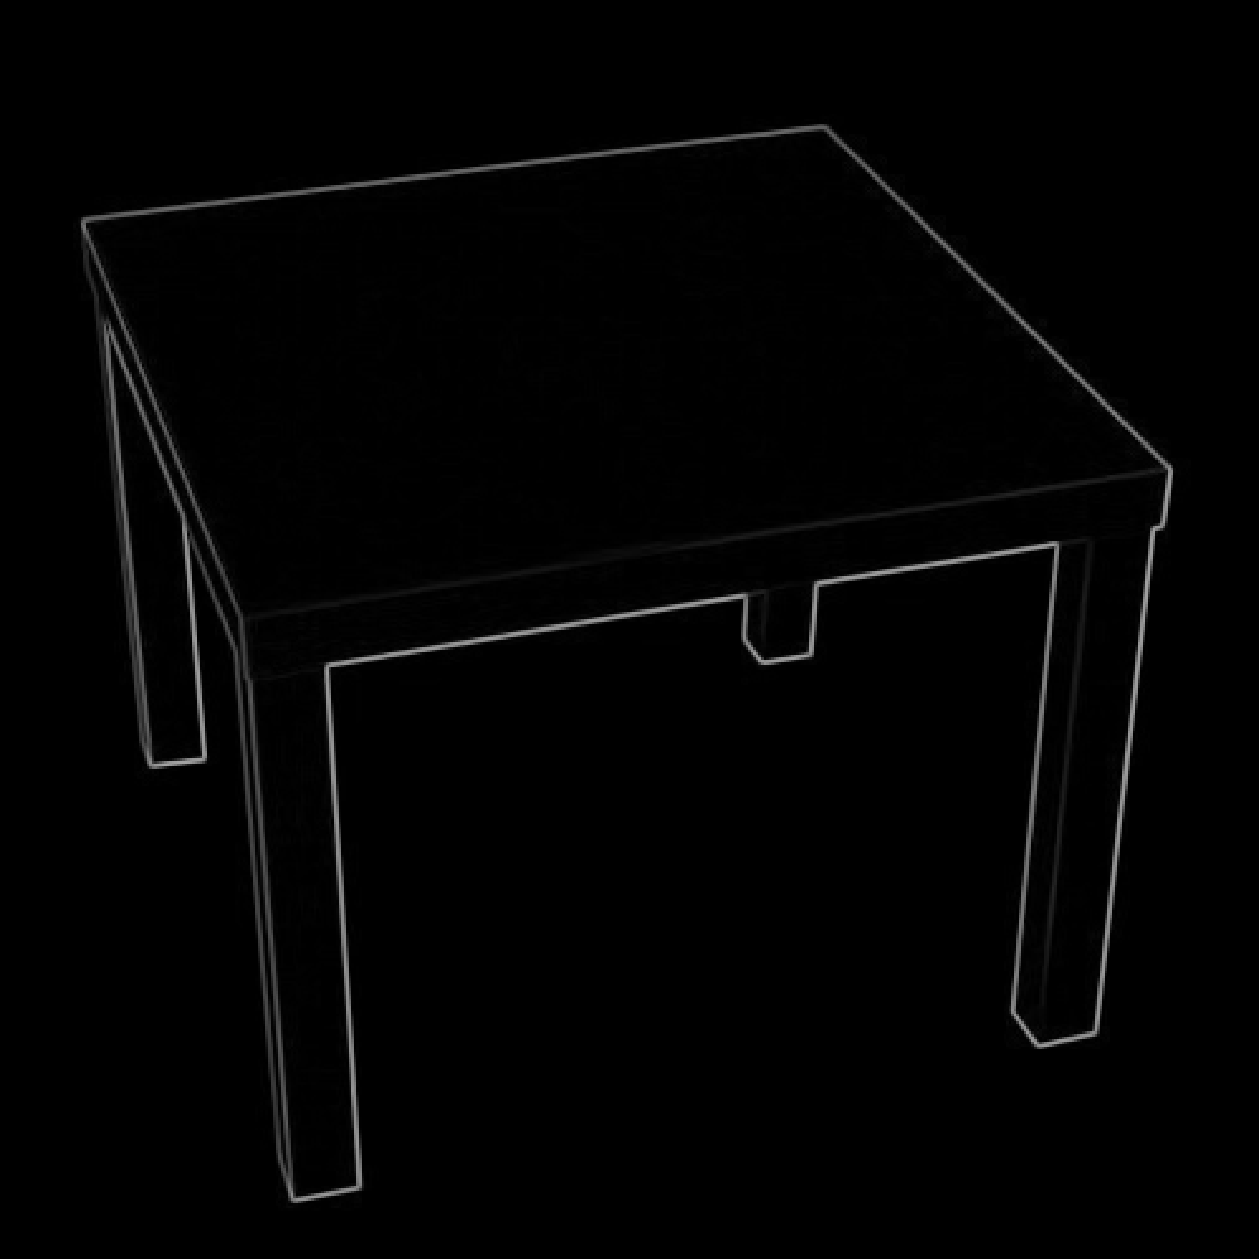
\includegraphics[height=6.5cm]{../code/img/desk_sobel.png}
	}
	\caption{桌子}
	\label{fig:desk}
\end{figure}

如图\ref{fig:desk}为来源互联网的一张桌子图片。图右为经过sobel算子提取边缘后的图片。

sobel算子如下:

\begin{equation}
\mathbf{G}_{\mathbf{x}}=\left[\begin{array}{rrr}{-1} & {0} & {+1} \\ {-2} & {0} & {+2} \\ {-1} & {0} & {+1}\end{array}\right] * \mathbf{A}
\end{equation}

\begin{equation}
\mathbf{G}_{\mathbf{y}}=\left[\begin{array}{ccc}{+1} & {+2} & {+1} \\ {0} & {0} & {0} \\ {-1} & {-2} & {-1}\end{array}\right] * \mathbf{A}
\end{equation}

Python代码如下:

\begin{lstlisting}[title={sobel算子}]
edges = filters.sobel(image)
\end{lstlisting}

\begin{figure}[ht]
	\centering
	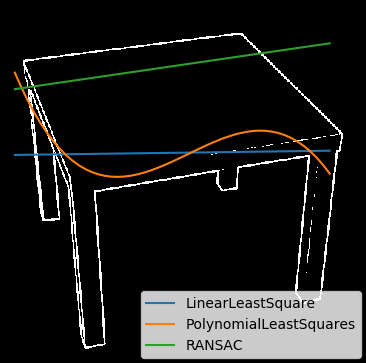
\includegraphics{../code/img/desk_LinearRegression.png}
	\caption{桌子图线性回归模型直线检测}
	\label{fig:desk-LinearRegression}
\end{figure}

如图\ref{fig:desk-LinearRegression}为最小二乘法和RANSAC对桌子图片直线检测的结果。

先对图像进行二值化,然后抽离出数据点,再进行回归预测。然而,对于这种众多离群点的数据,回归算法往往不能取得好的效果。一个可行的解决方法是把图片分为若干个部分,分别进行回归预测,但由于复杂这里并未实现。

\begin{figure}[ht]
	\centering
	\subfigure[threshold=100]{
		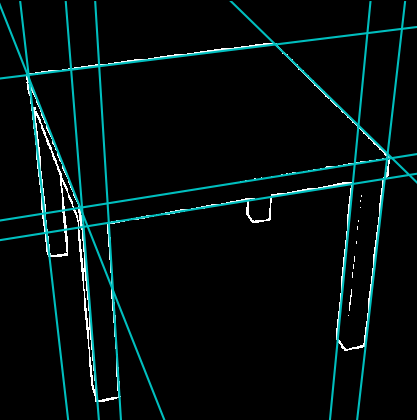
\includegraphics[height=6.5cm]{../code/img/desk_hough_line100.png}
		%\caption{fig1}
	}
	\quad
	\subfigure[threshold=250]{
		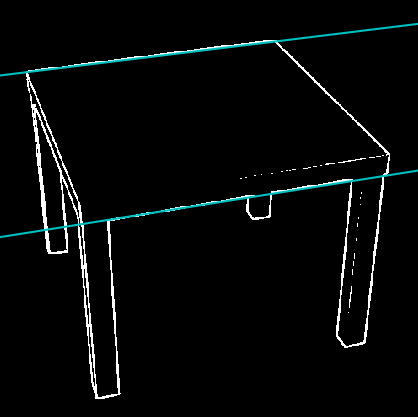
\includegraphics[height=6.5cm]{../code/img/desk_hough_line250.png}
	}
	\caption{桌子图霍夫直线检测}
	\label{fig:desk-hough-line}
\end{figure}

如图\ref{fig:desk-hough-line}为桌子图霍夫直线检测不同参数结果,效果良好。



























\clearpage
\begin{appendix}
	\section{完整源码}
	
	\lstinputlisting[title={LinearRegression.py}]{../code/LinearRegression.py}
	
	\lstinputlisting[title={LSD.py}]{../code/LSD.py}
	
	
\end{appendix}





























\end{document}

